At the end we have 21 docker containers that are database related. All of the Docker containers are on local network (localhost) in our case. In the table bellow, we can see the function they have.

\begin{center}
\begin{longtable}{ |m{5.5cm}|m{6cm}|m{1.5cm}| } 
 \hline
    Container name & Container description & Port \\ 
 \hline
 \hline
    mongo{\_}ReplicaSet1{\_}Node1 & Storage node 1 for replica set 1 & 40117\\ 
 \hline
    mongo{\_}ReplicaSet1{\_}Node2 & Storage node 2 for replica set 1 & 40127\\ 
 \hline
    mongo{\_}ReplicaSet1{\_}Node3 & Storage node 3 for replica set 1 & 40137\\ 
 \hline
    mongo{\_}ReplicaSet1{\_}Arbiter & Tie breaker for replica set 1 & 40147\\ 
 \hline
    mongo{\_}ReplicaSet1{\_}Backup & Backup node for replica set 1 & 40157\\ 
 \hline
 \hline
    mongo{\_}ReplicaSet2{\_}Node1 & Storage node 1 for replica set 2 & 40217\\ 
 \hline
    mongo{\_}ReplicaSet2{\_}Node2 & Container 1 for replica set 2 & 40227\\ 
 \hline
    mongo{\_}ReplicaSet2{\_}Node3 & Container 1 for replica set 2 & 40237\\ 
 \hline
    mongo{\_}ReplicaSet2{\_}Arbiter & Tie breaker for replica set 2 & 40247\\ 
 \hline
    mongo{\_}ReplicaSet2{\_}Backup & Backup node for replica set 2 & 40257\\ 
 \hline
 \hline
    mongo{\_}ReplicaSet3{\_}Node1 & Storage node 1 for replica set 3 & 40317\\ 
 \hline
    mongo{\_}ReplicaSet3{\_}Node2 & Storage node 2 for replica set 3 & 40327\\ 
 \hline
    mongo{\_}ReplicaSet3{\_}Node3 & Storage node 3 for replica set 3 & 40337\\ 
 \hline
    mongo{\_}ReplicaSet3{\_}Arbiter & Tie breaker for replica set 3 & 40347\\ 
 \hline
    mongo{\_}ReplicaSet3{\_}Backup & Backup node for replica set 3 & 40357\\ 
 \hline
 \hline
    mongo{\_}Config1 & Configuration server 1 & 27017\\ 
 \hline
    mongo{\_}Config2 & Configuration server 2 & 27017\\ 
 \hline
    mongo{\_}Config3 & Configuration server 3 & 27017\\ 
 \hline
 \hline
    mongo{\_}Shard1 & Main router & 27019\\ 
 \hline
    mongo{\_}Shard2 & Backup router 1 & 27020\\ 
 \hline
    mongo{\_}Shard3 & Backup router 2 & 27021\\ 
 \hline
\caption{Containers used described}
\end{longtable}
\end{center}

\begin{figure}[H]
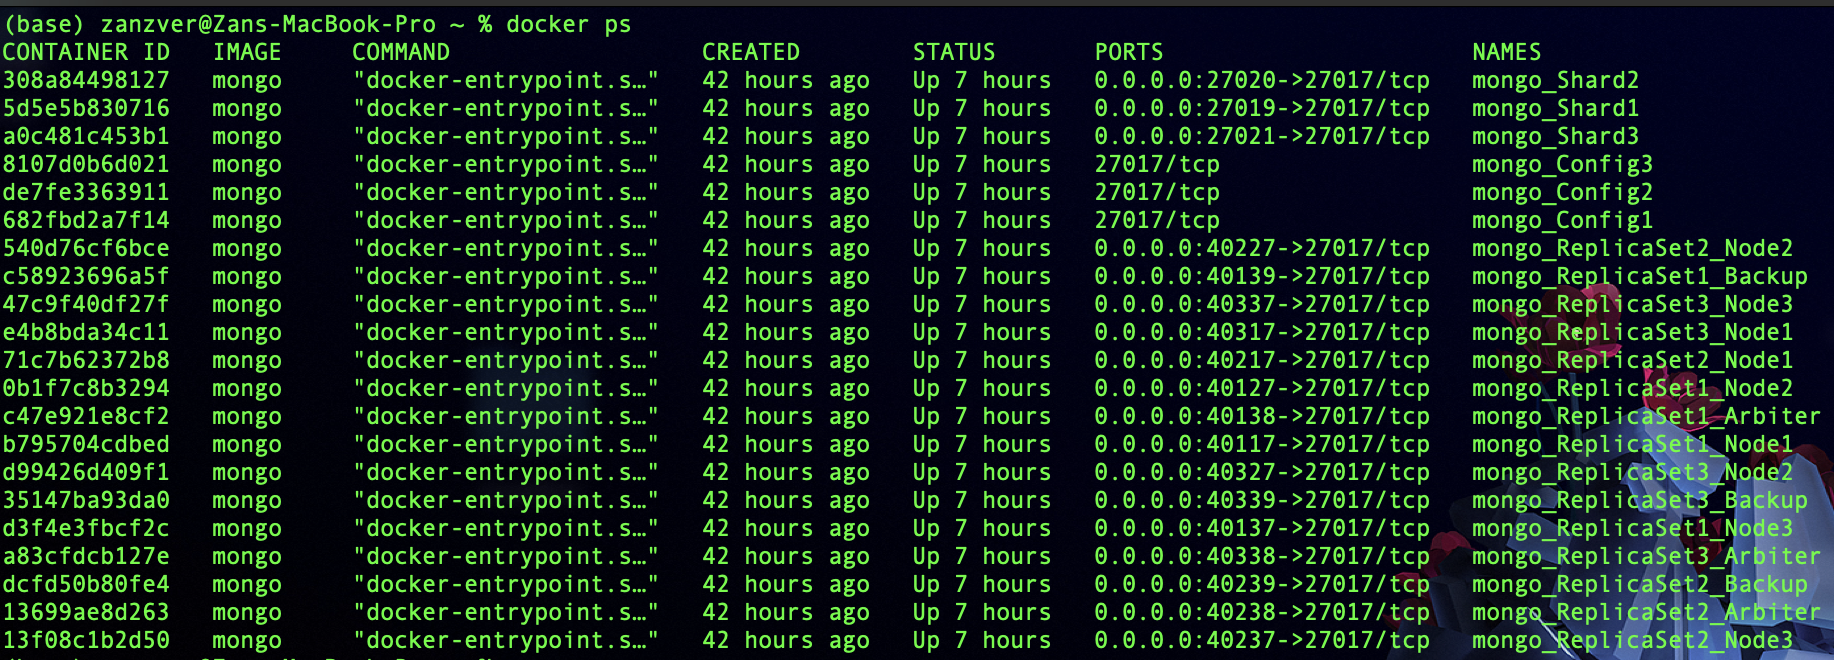
\includegraphics[scale=0.45]{img/allDockerContainers.png}
\centering
\caption{Containers displayed in terminal}
\end{figure}